% !TEX options=--shell-escape
\documentclass[12pt]{article}
\usepackage[utf8]{inputenc}
\usepackage{lipsum}
\usepackage{afterpage}
\usepackage{mathtools}
\usepackage{xcolor}
\usepackage[12pt]{extsizes}
\usepackage[english,russian]{babel}
\usepackage{cite}
\usepackage{minted}
\usepackage{amsmath, esint, setspace, fancyhdr, amsfonts, bookmark, blindtext}
\usepackage{graphicx}
\usepackage{subfigure}
\usepackage{titlesec}

\graphicspath{{Figures/}}
\DeclareGraphicsExtensions{.pdf,.png,.jpg}
\usemintedstyle{tango}
\definecolor{dhscodebg}{rgb}{0.95,0.95,0.95}


\setlength{\textheight}{8in}
\setlength{\textwidth}{6.6in}
\setlength{\headheight}{0in}
\setlength{\headsep}{0.2in}
\setlength{\topmargin}{0in}
\setlength{\oddsidemargin}{0in}
\setlength{\evensidemargin}{0in}
\setlength{\parindent}{.3in}

\doublespacing
\renewcommand{\baselinestretch}{1.4} 

\begin{document}
\begin{titlepage}

\begin{center}
Санкт-Петербургский политехнический университет Петра Великого\\
Институт прикладной математики и механики\\
Кафедра прикладной математики\\
\end{center}


\vspace{2.5cm}

\begin{center}
{\large {\bfseries СВОДНЫЙ ОТЧЕТ}}\\

\bigskip \bfseries{Тема:} {\bfseries \emph{Многомерные распределения.\\ Оценки характеристик распределений}}
\end{center}

\vspace{1.5cm}

\begin{flushleft}
Направление: 01.03.02 Прикладная математика и информатика

\vspace{1.5cm}

Выполнил студент гр. 33631/4 \hfill{Камалетдинова Ю.} \\ 

\vspace{0.5cm} Преподаватель \hfill{Баженов А.}
\vspace{1cm}

\end{flushleft}

\vspace{2.7cm}

\begin{center}
Санкт-Петербург\\
2019
\end{center}

\end{titlepage}

\newcommand{\threeimage}[4]{
\begin{figure}[h!]  
    \centering 
    \subfigure[]{
        \includegraphics[width=0.3\linewidth, height=0.25\linewidth]{#1} 
        \label{fig:f_ #1} }  
        %\hspace{4ex}
    \subfigure[]{
    \includegraphics[width=0.3\linewidth, height=0.25\linewidth]{#2} 
    \label{fig:f_ #2} }
   % \hspace{4ex}
    \subfigure[]{ 
        \includegraphics[width=0.3\linewidth, height=0.25\linewidth]{#3} 
        \label{fig:f_ #3} }  
    \caption{Выборки из #4 объемом: 
    \subref{fig:f_ #1} 20; 
    \subref{fig:f_ #2} 60; 
    \subref{fig:f_ #3} 100} 
    \label{fig:f_ #1#2#3}
\end{figure}}

\newcommand{\triplethreeimage}[4]{
\begin{figure}[h!]  
    \centering 
    \subfigure[]{
        \includegraphics[width=.83\linewidth, height=.3\linewidth]{#1} 
        \label{fig:f_ #1} }\\  
    %\hspace{4ex}
    \subfigure[]{
        \includegraphics[width=.83\linewidth, height=.3\linewidth]{#2} 
        \label{fig:f_ #2} }\\
    %\hspace{4ex}
    \subfigure[]{ 
        \includegraphics[width=.83\linewidth, height=.3\linewidth]{#2} 
        \label{fig:f_ #3} }  
    \caption{Для выборок из #4 объемом: 
    \subref{fig:f_ #1} 20; 
    \subref{fig:f_ #2} 60; 
    \subref{fig:f_ #3} 100} 
    \label{fig:f_ #1#2#3}
\end{figure}}

\tableofcontents
\addtocontents{toc}{~\hfill\par}
\vfill ~
\setcounter{section}{0}


%%%%%%%%%%%%%%%%%%%%%%%%%%%%%%%%%%%%%%%%%%

\newpage 
\section*{Постановка задачи}
\addcontentsline{toc}{section}{Постановка задачи}

\indent{\indentДанная группа лабораторных работ посвящена рассмотрению одномерных распределений. Выделим основные задачи:}
\begin{itemize}
	\item Исследовать такой способ представления набора статистических данных как гистограмма. Сгенерировать выборки разного размера для заданных распределений, построить гистограммы и сделать выводы о взаимосвязи функции плотности распределения и функции гистограммы.
	\item{Вычислить некоторые из характеристик положения $N = 1000$ раз для выборок объемами $n = 20, 50, 100$ и проанализировать полученные результаты. Также необходимо установить, в каком соотношении находятся вычисленные характеристики для каждого из распределений, приведенных ниже
	\begin{equation}
		\label{dist:1}
		N(x, 0, 1) = \frac{1}{\sqrt{2\pi}}e^{-\frac{x^2}{2}} \;\text{-- стандартное нормальное}
	\end{equation}
	 
	\begin{equation}
		C(x, 0, 1) = \frac{1}{\pi(1 + x^2)} \;\text{-- Коши} \label{dist:2}
	\end{equation}

	\begin{equation}
		L(x, 0, \frac{1}{\sqrt{2}}) = \frac{1}{\sqrt{2}}e^{{-\sqrt{2}|x|}} \;\text{-- Лаплас} \label{dist:3}
	\end{equation}

	\begin{equation} 
		U(x, -\sqrt{3}, \sqrt{3}) = 
	    \begin{cases}
	        \frac{1}{2\sqrt{3}}, \: |x| \leq \sqrt{3}\\
	        \;\; 0, \:\:\:|x| > \sqrt{3}
	    \end{cases}
	    \;\text{-- равномерное} \label{dist:4}
	\end{equation}

	\begin{equation}
	    P(\lambda) = \frac{e^{-\lambda}}{k!}\lambda^k \;\text{-- Пуассон} \label{dist:5}
	\end{equation}

	\indent{Приведем формулы для вычисления характеристик положения}

	\begin{equation}
		\label{char:1}
		\overline{x} = \overline{x_n} = \frac{1}{n} \sum_{i=1}^{n}{x_i} \;\text{-- выборочное среднее}
	\end{equation}
	\begin{equation} 
		med \; x = 
	    \begin{cases}
	        \;\;\; x_{(k+1)}, \:\;\;\; n = 2k + 1 \\
	        \frac{x_{(k)} + x_{(k+1)}}{2}, \; n = 2k
	    \end{cases}
	    \;\text{-- медиана} \label{char:2}
	\end{equation}

	\begin{equation}
		\label{char:3}
		z_R = \frac{x_{(1)} + x_{(n)}}{2}  \;\text{-- полусумма экстремальных значений}
	\end{equation}

	\begin{equation}
		\label{char:4}
		z_Q = \frac{Q_1 + Q_3}{2}  \;\text{-- полусумма квартилей}
	\end{equation}

	\begin{equation}
		\label{char:5}
		z_{tr} = \frac{1}{n - 2r} \sum_{i = r + 1}^{n - r}{x_{(i)}}  \;\text{-- усеченное среднее}
	\end{equation}

	\indent{\underline{Замечание:} $r$ -- число наблюдений, оставшихся после усечения в характеристике \eqref{char:5}, $r = \alpha n$, где $\alpha$, как правило, равняется $0.1$. В таком случае мы не вовлекаем $10$\% наибольших и $10$\% наименьших значений в вычисление усеченного среднего.} }
	\item Cгенерировать выборки размерами $n = 20, 100$ и построить для них боксплот Тьюки. Для каждого распределения определить процент выбросов экспериментально, сгенерировав выборку из распределения $N =1000$ раз и вычислив средний процент выбросов, а затем сравнить с результатами, полученными теоретически. Рассматриваемые законы распределения – \eqref{dist:1}, \eqref{dist:2}, \eqref{dist:3}, \eqref{dist:4}, \eqref{dist:5}

	\item Построить эмпирические функции распределения и ядерные оценки плотностей для распределений \eqref{dist:1}, \eqref{dist:2}, \eqref{dist:3}, \eqref{dist:4}, \eqref{dist:5} с параметром $\lambda = 2$ на выборках размером $N = 20,\;60,\;100$ на отрезке $[-4,\;4]$, а также сделать выводы о данных оценках законов распределений. 
\end{itemize}
\indent{ }

%%%%%%%%%%%%%%%%%%%%%%%%%%%%%%%%%%%%%%%%%%

\section*{Описание методов}
\addcontentsline{toc}{section}{Описание методов}

\textbf{\indentГистограммы} 

\indent{ Для построения гистограммы разобьем множество возможных значений $\xi$ выбоки на непересекающиеся интервалы $\Delta_j = [t_j, t_{j+1}), \; j=\overline{0, m}; \; t_0=-\infty,\; t_{m+1}=+\infty$. Количество элементов $X$ выборки из объема $n$, попавших в интервал $\Delta_j$, обозначим через $v_j$, то есть $v_j = \sum_{i=1}^{n}{I(X_i \in \Delta_j)}$. По теореме Бернулли при $n\to\infty$}

\begin{equation}
    \label{1_eq:1}
    v_j/n \to P(\xi \in \Delta_j) = \int_{\Delta_j}f(u)du = |\Delta_j|f(c), \; c \in \Delta_j
\end{equation}

\indent{ Кусочно-постоянная функция, приведенная ниже, есть нормализованная гистограмма}

\begin{equation}
    \label{1_eq:2}
	f_n(t)= \frac{v_j}{n|\Delta_j|}, \; t \in \Delta_j, \; j = \overline{1, m}
\end{equation}

\indent{ Итак, гистограмма является статистическим аналогом функции плотности распределения и функции распределения. Формулы \eqref{1_eq:1}, \eqref{1_eq:2} указаны в пособии \cite{ms_1}.} \\

\textbf{Выявление выбросов} 

\indent{ \textit{Выброс} -- это некое наблюдение, которое нехарактерно далеко удалено от других значений в общей случайной выборке. В некотором смысле, это определение оставляет на усмотрение наблюдателя решение вопроса о том, что будет считаться выбросом. } 

\indent{ Боксплот является удобным графическим способом описания поведения данных как в середине, так на концах распределения. Боксплот визуализирует положение медианы, нижнего и верхнего квартилей. Первый квартиль $Q_1$ определяется как медиана части выборки до медианного элемента всей выборки, третий квартиль $Q_3$ -- медиана части выборки после медианного элемента всей выборки.} 

\indent{На графике присутствуют усы, границы которых определяются формулами}
\begin{equation}
    \label{3_eq:1} 
    x_L = max(x_{(1)},\; Q_1 - 1.5 \cdot IQR)\text{ -- нижняя граница уса}
\end{equation}

\begin{equation}
    \label{3_eq:2} 
    x_U = min(x_{(n)},\; Q_3 + 1.5 \cdot IQR)\text{ -- верхняя граница уса}
\end{equation}

\begin{equation}
    \label{3_eq:3} 
    IQR = Q_3 - Q_1   \text{ -- интерквартильная широта}
\end{equation}

\indent{Будем считать элемент $x_i$ выбросом, если $x_i \notin [x_L, x_U]$}

\indent{Для сравнения теоретических и практических результатов вычислим квартили для непрерывных распределений. Квартили однозначно определяются уравнением}

\begin{equation}
    \label{3_eq:4}
    F_X(x_{\alpha}) = \alpha \text{,\;\;} \alpha = \left\{ \frac{1}{4}, \; \frac{3}{4} \right\}
\end{equation}

\indent{Искомые квартили можно выразить, найдя обратную функцию к функции распределения.}

\indent{Вычисление доли выбросов будем производить по формуле}
\begin{equation}
\label{3_eq:5}
    p_{outliers} = \frac{\sum_{i}^{} x_i}{\sum_{j = 1}^{n} x_j}, \; i: x_i \notin [x_L, x_U] 
\end{equation} 

\textbf{Ядерные оценки плотностей и функции плотностей распределения} 

\indent{ Пусть имеется некоторая выборка объемом $n: \; x_1, \ldots, \; x_n; \; x_i \in \mathbb{R}$. Эмпирической функцией распределения называют}

\begin{equation} 
    \hat{F_n}(x) = \frac{1}{n} \sum_{i=1}^{n}{u(x - x_i)}, \; \label{4_eq:1} \text{где}
\end{equation}

\begin{equation} 
    u(z) = 
    \begin{cases}
        1, \; z \geq 0 \\
        0, \; z \leq 0
    \end{cases}
    \text{ – фунция Хевисайда} 
    \label{4_eq:2}
\end{equation}

Ядерная оценка плотности определяется формулой:
\begin{equation}
    \hat{f}_{n, h_n}(x)=\frac{1}{nh_n} \sum_{i=1}^{n}{K \left(\frac{x - x_i}{h_n}\right)}, \; \label{4_eq:3} \text{где $K(u)$ – ядро, $h = h_n$ – параметр сглаживания}
\end{equation}

Ядро $K(u)$  – это вещественнозначная функция со следующими свойствами:

\begin{enumerate}
    \item $K(u) \geq 0$
    \item $K(-u) = K(u)$
    \item $\displaystyle \int_{-\infty}^{+\infty}{K(u)du} = 1$
\end{enumerate}
\indent{\indent Ядерная оценка плотности сглаживает каждый элемент выборки до плавного участка, форма которого определяется функцией ядра $K(u)$. Затем функция суммирует все участки, чтобы получить оценку плотности. В данной работе будем использовать ядро Гаусса, заданное формулой}

\begin{equation}
    K(u) = \frac{1}{\sqrt{2\pi}}e^{-\frac{x^2}{2}} \label{4_eq:4}
\end{equation}

%%%%%%%%%%%%%%%%%%%%%%%%%%%%%%%%%%%%%%%%%%

\section*{Реализация}
\addcontentsline{toc}{section}{Реализация}
\indent{ \indentДля выполнения поставленных задач будем пользоваться библиотеками для языка Python: \textit{numpy, scipy} -- расчеты, законы распределения вероятностей; \textit{matplotlib, seaborn} -- визуализация результатов. Опишем ход работы для каждой задачи:}
\begin{itemize}
	\item { Гистограммы
	\begin{itemize}
		\item Производим построение графика теоретической функции распределения
		\item При помощи метода \texttt{.rvs} берется выборка размера n из распределения с заданными параметрами
		\item Определяем границы области интересующих нас значений и разделяем на равные интервалы (\textit{bins})
		\item Строим гистограммы, представляющие собой столбцы высотой, пропорциональной числу попавших в их ширину значений
		\item Нормируем гистограммы и отрисовываем теоретическую функцию распределения в одних осях  
	\end{itemize} }
	\item {Характеристики положения
	\begin{itemize}
	    \item Задаем распределение с заданными параметрами 
	    \item Генерирем случайные выборки из распределений размерами $n = 20, 50, 100$
	    \item Для каждого из распределений вычисляем характеристики положения $N = 1000$ раз
	    \item Вычисляем математическое ожидание и дисперсию для каждой вычисленной характеристики по формулам:
	    \begin{equation}
	    \label{moment:1}
	      E(z) = \overline{z} = \frac{1}{N}\sum_{i=1}^{N}{z_i}
	    \end{equation}
	    \begin{equation}
	    \label{moment:2}
	      D(z) = \overline{z^2} - (\overline{z})^2
	    \end{equation}
	\end{itemize}}
	\item {Выявление выбросов
	\begin{itemize}
	    \item Задаем распределение с заданными параметрами 
	    \item Генерируем случайные выборки из распределений размерами $n = 20, 100$
	    \item Для каждого из распределений вычисляем доли выбросов $N = 1000$ раз
	    \item Вычисляем теоретические квартили при помощи метода \texttt{.ppf($\alpha$)} (percent point function) - функция, обратная функции распределения, вычисляем доли выбросов с использованием данных квартилей
	    \item Усредняем полученные суммы долей выбросов, разделив на $N = 1000$ 
	\end{itemize}}
	\item {Ядерные оценки плотностей и эмпирические распределения
	\begin{itemize}
	    \item Задаем распределение с заданными параметрами 
	    \item Генерируем случайные выборки из распределений объемами $n = 20, \; 60, \; 100$
	    \item Для отсортированных выборок из распределений задаем вектор значений $y = [\frac{1}{n}, \frac{2}{n}, \ldots, 1]$ и строим ступенчатый график - эмпирическую функцию распределения 
	    \item По формулам \eqref{4_eq:3}, \eqref{4_eq:4} вычисляем ядерные оценки плотностей для параметров сглаживания $h$ для всех выборок и строим графики 
	\end{itemize}}
\end{itemize}

%%%%%%%%%%%%%%%%%%%%%%%%%%%%%%%%%%%%%%%%%%

\newpage
\section*{Результат}
\addcontentsline{toc}{section}{Результат}

\textbf{Нормальное распределение} с параметрами 0, 1
\begin{figure}[h!]
	\centering
	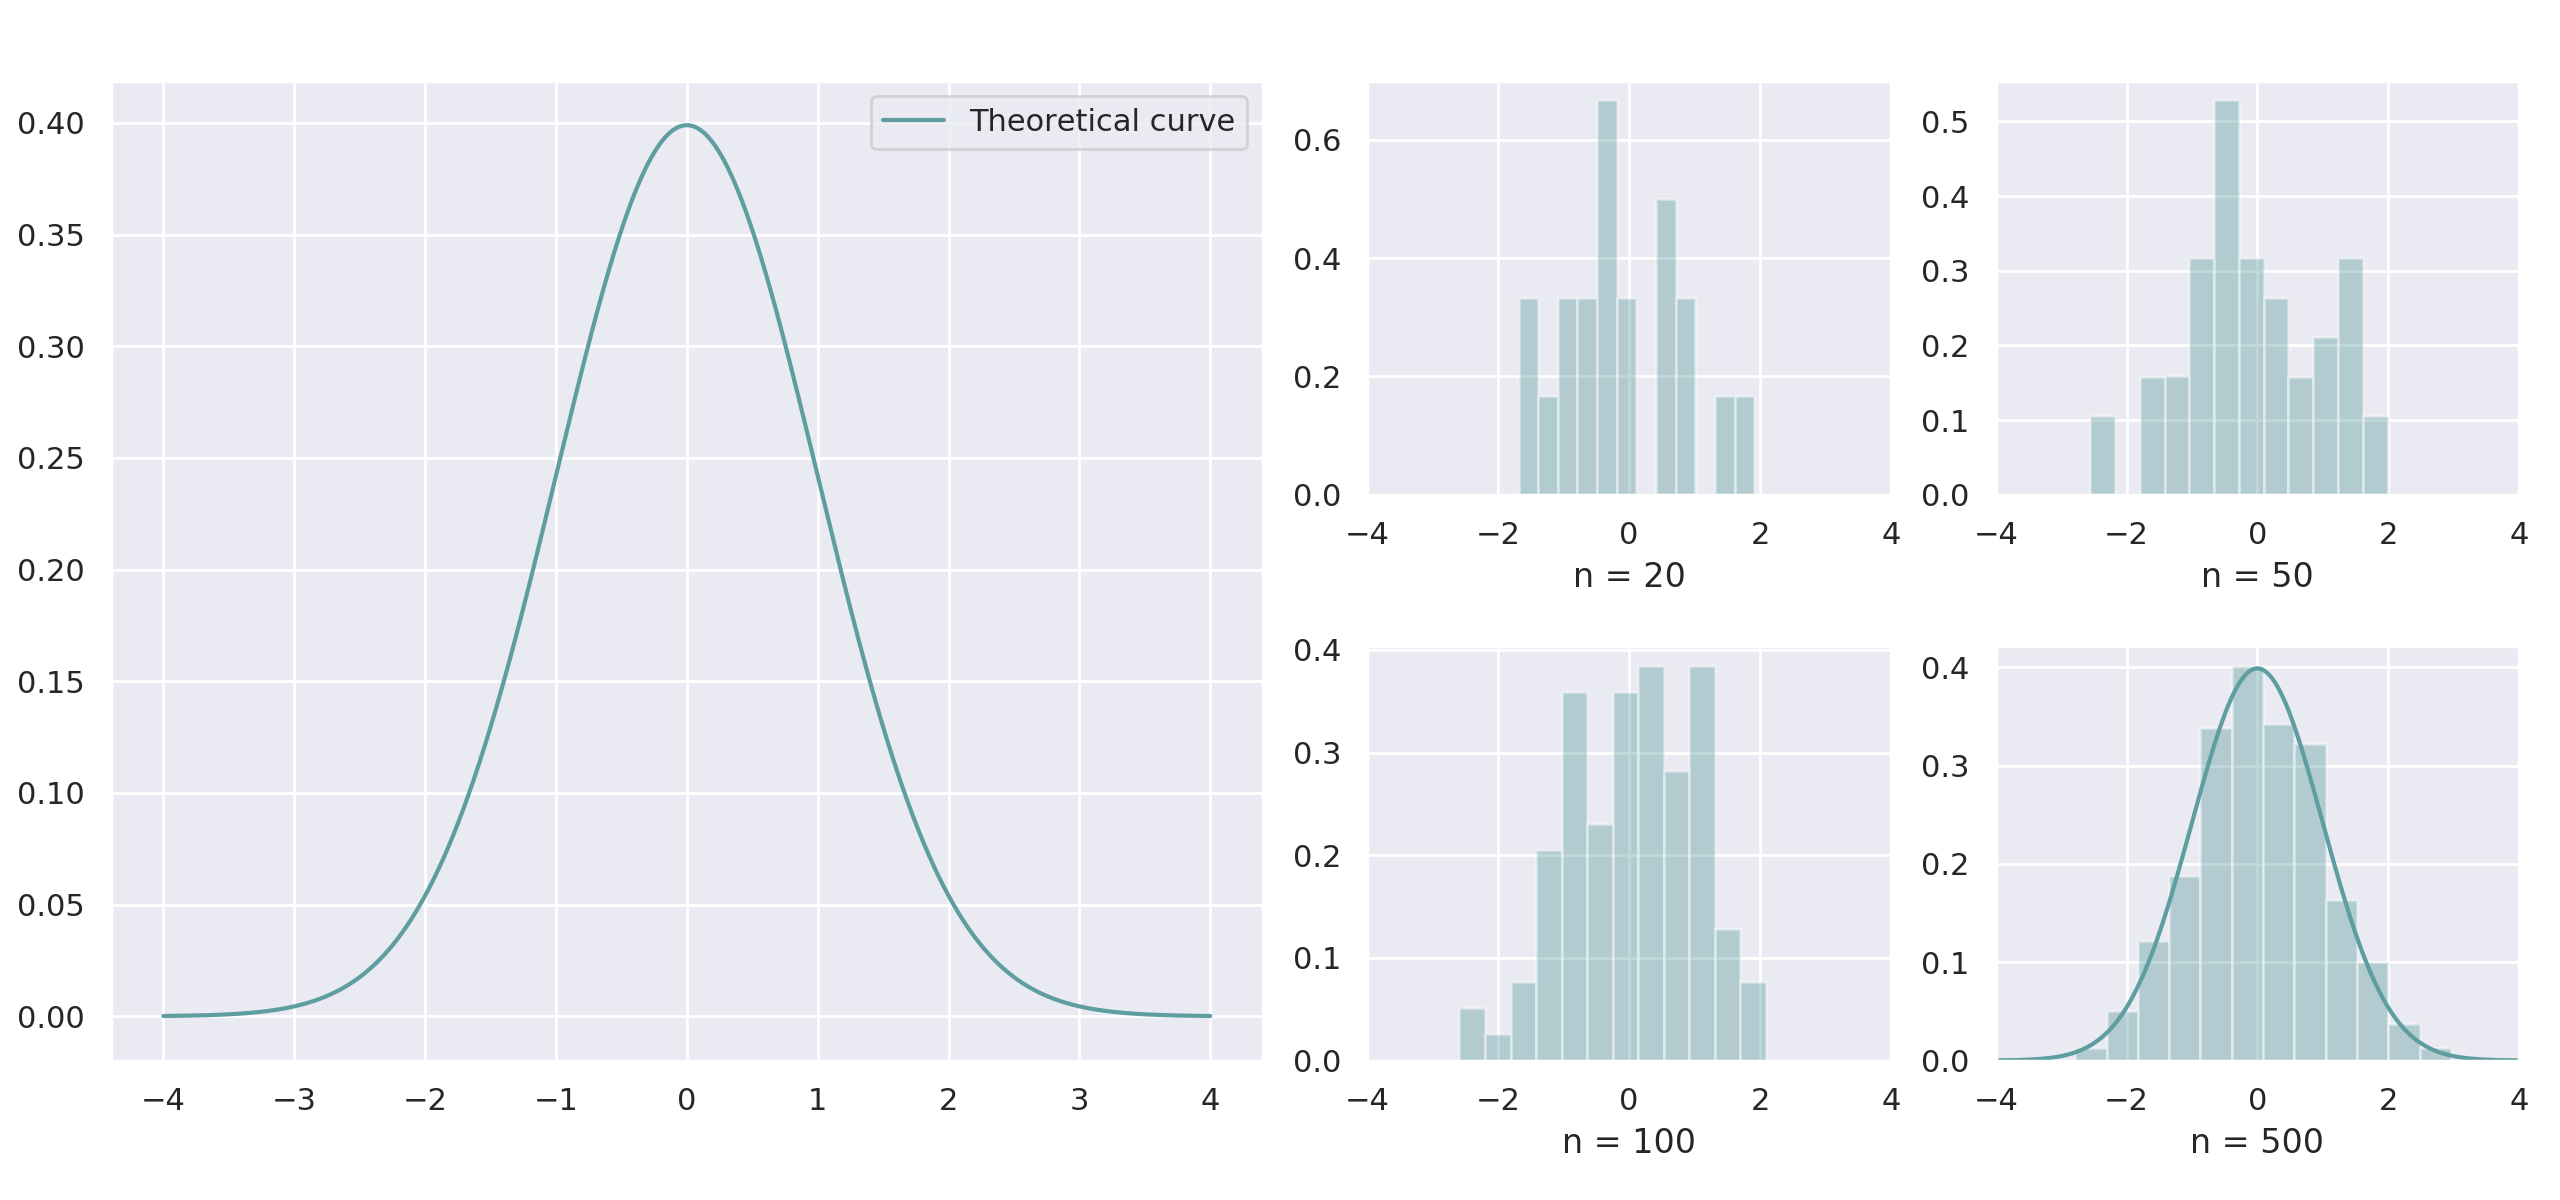
\includegraphics[width=16.cm, height=7.8cm]{norm_th}
	\caption{Гистограмма нормального распределения}
	\label{1_pic:1}
\end{figure}

\begin{table}[h!]
	\begin{tabular}{ | c | c | c | c | c | c |}
	\hline
	$n = 20$ & $\overline{x}$ & $med\;x$ & $z_R$ & $z_Q$ & $z_{tr}$ \\ \hline
	$E(z)$ & 0.0041 & 0.0053 & 0.0005 & 0.0046 & 0.0054 \\ \hline
	$D(z)$ & 0.0511 & 0.0753 & 0.1405 & 0.0586 & 0.0542 \\ \hline
	\end{tabular}
	\\
	\\ \\
	\begin{tabular}{ | c | c | c | c | c | c |}
	\hline
	$n = 50$ & $\overline{x}$ & $med\;x$ & $z_R$ & $z_Q$ & $z_{tr}$ \\ \hline
	$E(z)$ & 0.0013 & -0.0004 & 0.0170 & 0.0003 & -0.0010 \\ \hline
	$D(z)$ & 0.0211 & 0.0313 & 0.1146 & 0.0251 & 0.0222 \\ \hline
	\end{tabular}
	\\ 
	\\ \\
	\begin{tabular}{ | c | c | c | c | c | c |}
	\hline
	$n = 100$ & $\overline{x}$ & $med\;x$ & $z_R$ & $z_Q$ & $z_{tr}$ \\ \hline
	$E(z)$ & 0.0028 & 0.0026 & 0.0037 & 0.0034 & 0.0023 \\ \hline
	$D(z)$ & 0.0100 & 0.0152 & 0.0887 & 0.0122 & 0.0106 \\ \hline
	\end{tabular}
	\caption*{Таблицы моментов 1-го и 2-го порядков}
\end{table}

\indent{Соотношение дисперсий при $n = 100$: $\;\overline{x} < z_{tr} < z_Q < med\;x < z_R$} 

\begin{center}
    \begin{tabular}{ c | c | c }
        $$ & Практическая доля выбросов & Теоретическая доля выбросов  \\ \hline
        $n = 20$ & 0.022 & 0.007 \\ \hline
        $n = 100$ & 0.009 & 0.007 \\ 
    \end{tabular}
\end{center}

\begin{figure}[h!]
	\centering
	\center{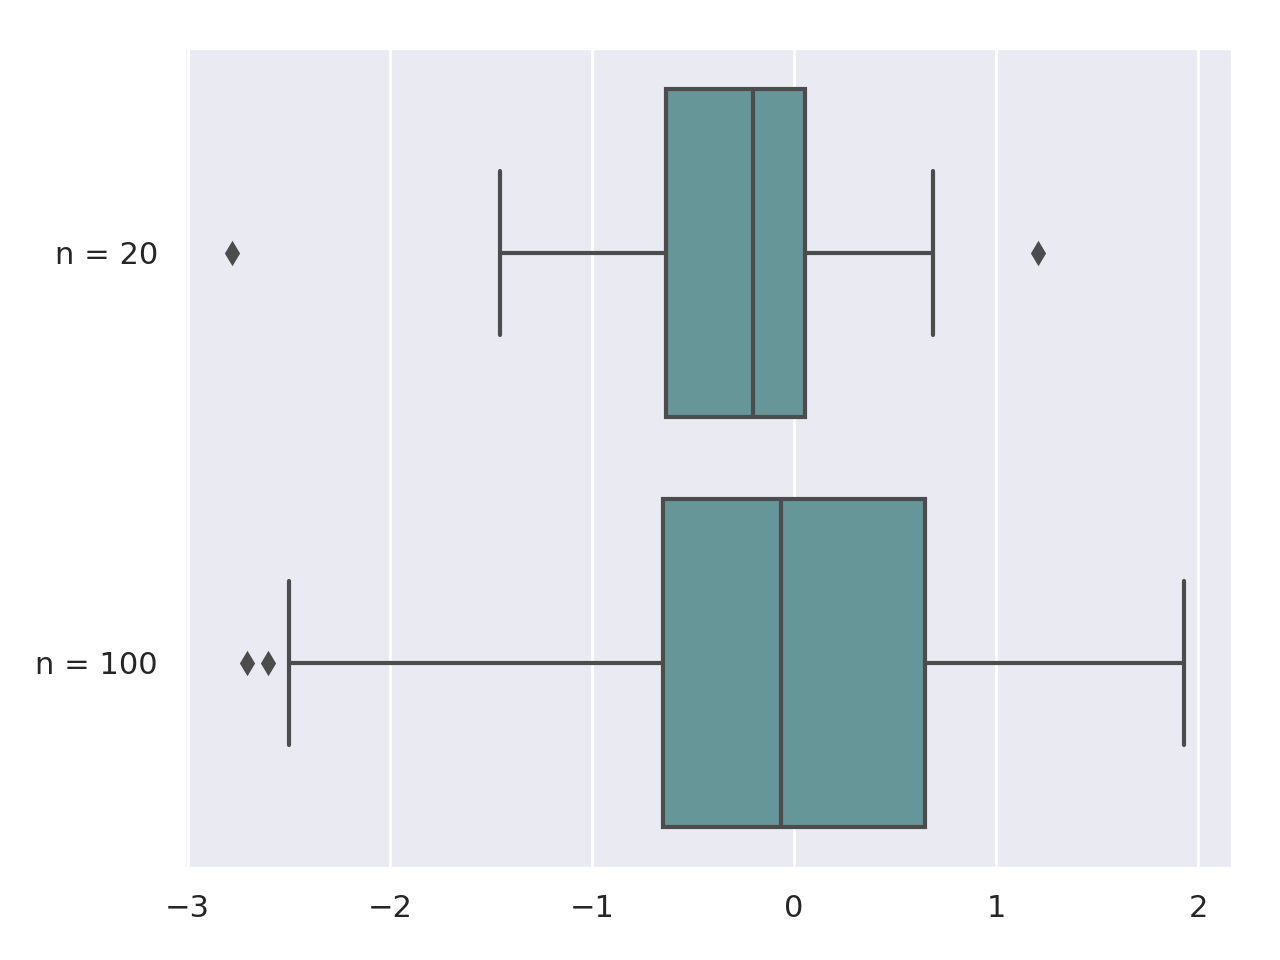
\includegraphics[width=12.cm, height=9.cm]{norm}}
	\label{1_pic:2}
	\caption{Боксплот Тьюки для выборок из нормального распределения}
\end{figure}

\threeimage{em_norm_20}{em_norm_60}{em_norm_100}{нормального распределения}
\triplethreeimage{ker_norm_20}{ker_norm_60}{ker_norm_100}{нормального распределения}
\newpage
\textbf{Равномерное распределение} на отрезке $[-\sqrt{3}, \sqrt{3}]$
\begin{figure}[h!]
\centering
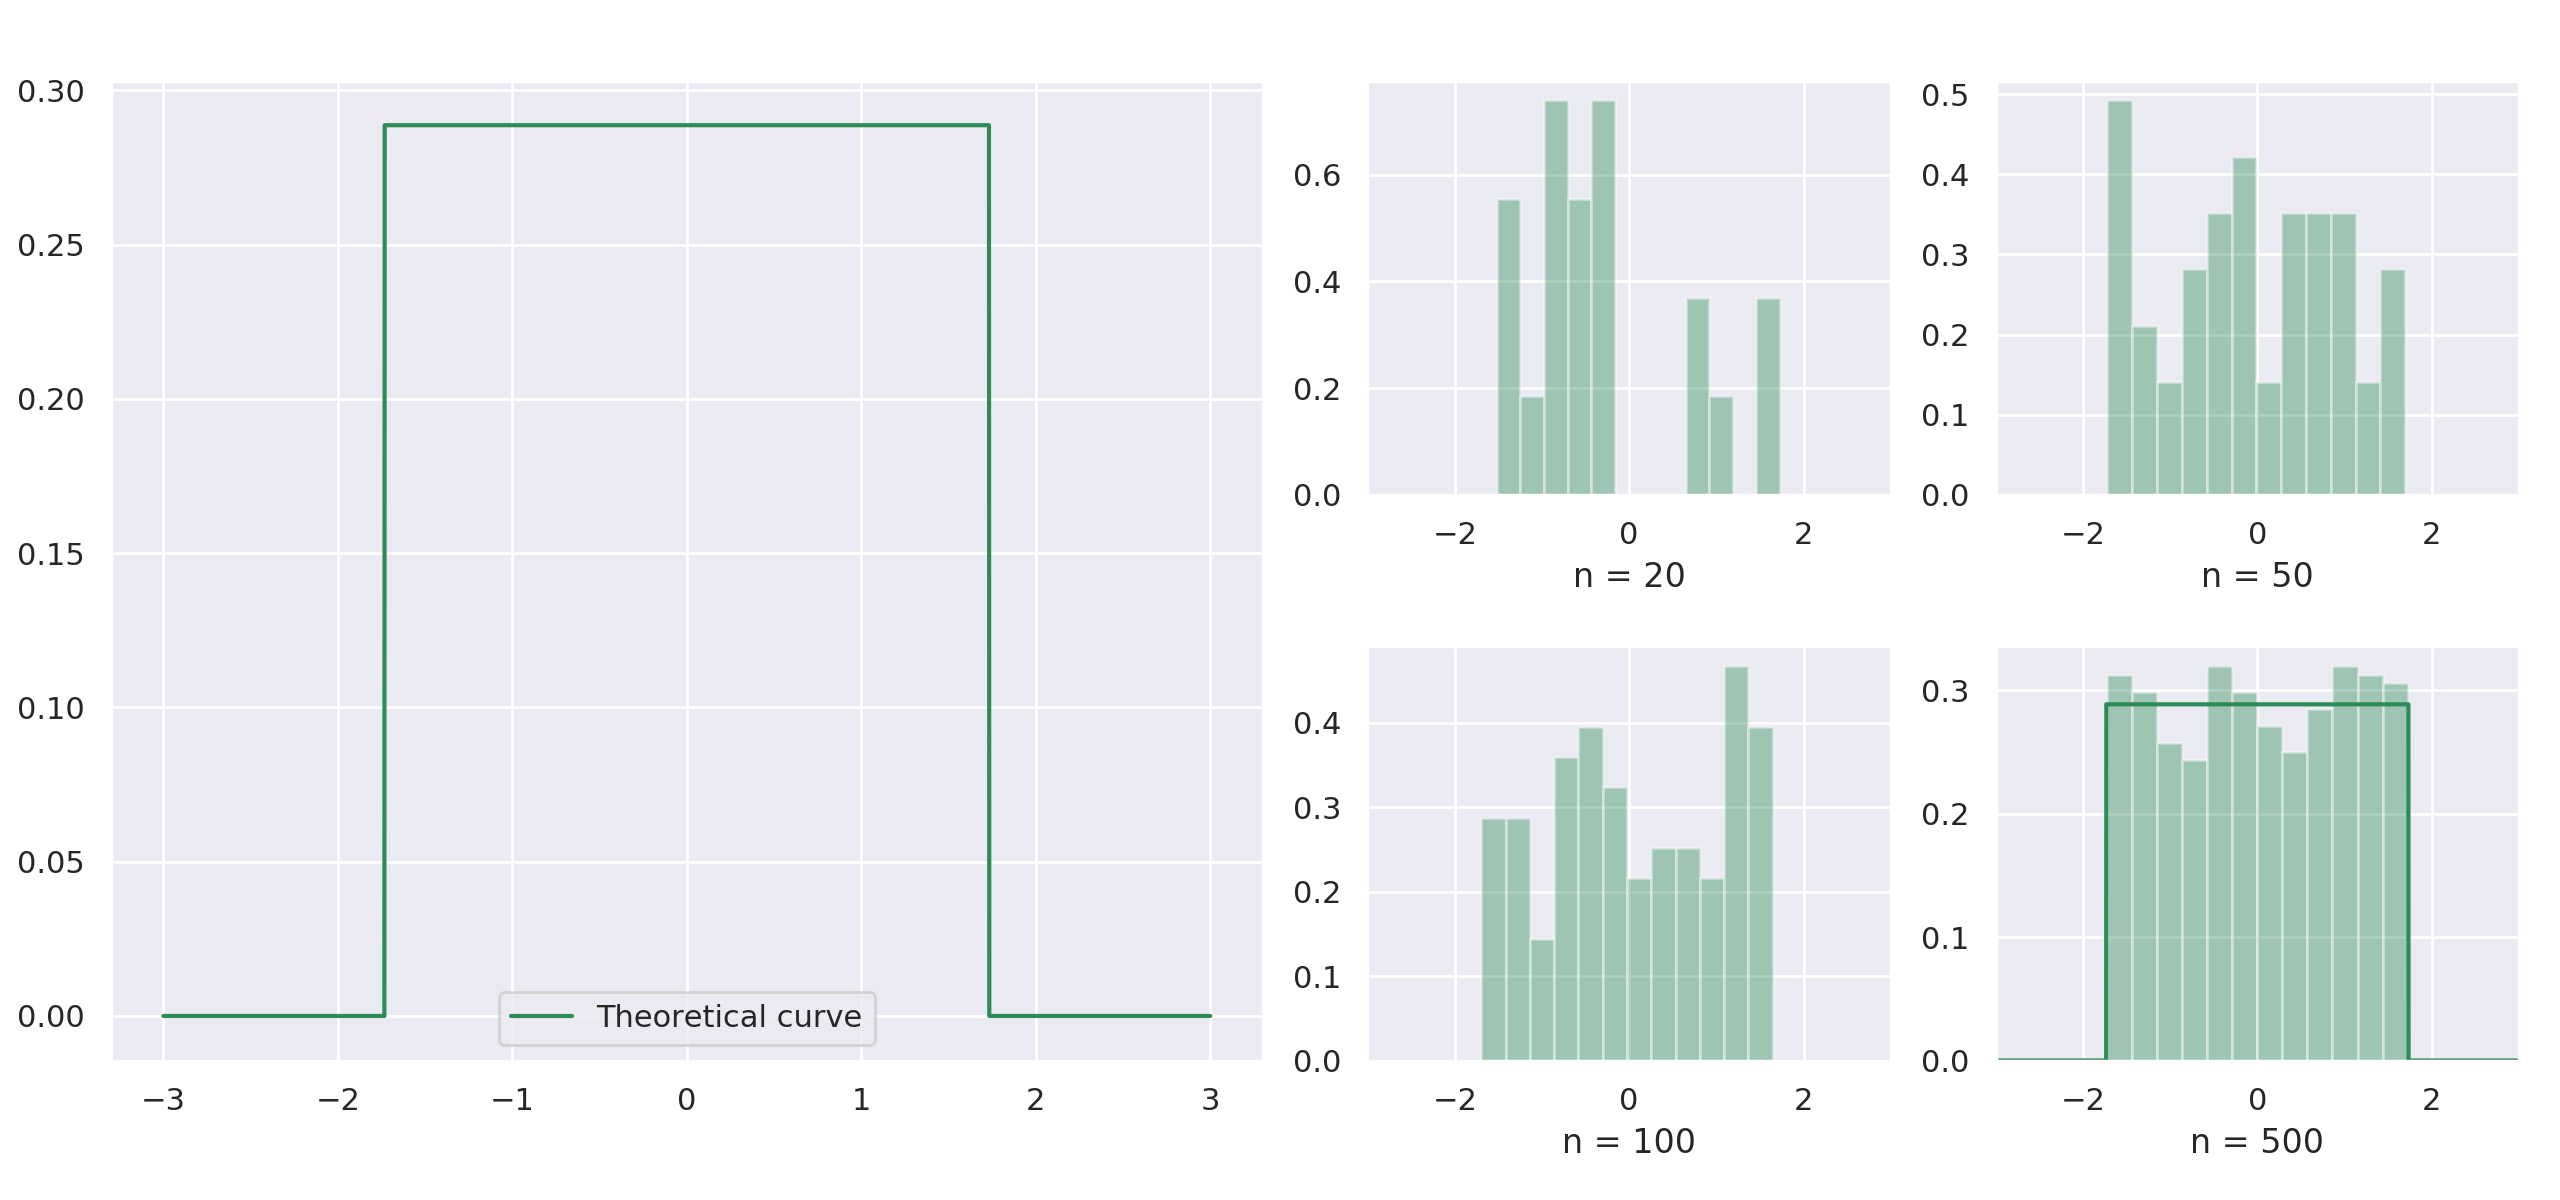
\includegraphics[width=16.cm, height=7.8cm]{uniform_th}
	\caption{Гистограмма равномерного распределения}
	\label{2_pic:1}
\end{figure}

\begin{table}[h!]
	\begin{tabular}{ | c | c | c | c | c | c |}
	\hline
	$n = 20$ & $\overline{x}$ & $med\;x$ & $z_R$ & $z_Q$ & $z_{tr}$ \\ \hline
	$E(z)$ & -0.0068 & -0.0119 & 0.0011 & -0.0113 & -0.0082 \\ \hline
	$D(z)$ & 0.0554 & 0.1404 & 0.0141 & 0.0728 & 0.0742 \\ \hline
	\end{tabular}
	\\
	\\ \\ 
	\begin{tabular}{ | c | c | c | c | c | c |}
	\hline
	$n = 50$ & $\overline{x}$ & $med\;x$ & $z_R$ & $z_Q$ & $z_{tr}$ \\ \hline
	$E(z)$ & 0.0032 & 0.0049 & -0.0004 & 0.0035 & 0.0040 \\ \hline
	$D(z)$ & 0.0209 & 0.0582 & 0.0022 & 0.0304 & 0.0288 \\ \hline
	\end{tabular}
	\\
	\\ \\ 
	\begin{tabular}{ | c | c | c | c | c | c |}
	\hline
	$n = 100$ & $\overline{x}$ & $med\;x$ & $z_R$ & $z_Q$ & $z_{tr}$ \\ \hline
	$E(z)$ & 0.0015 & 0.0015 & 0.0011 & 0.0017 & 0.0019 \\ \hline
	$D(z)$ & 0.0098 & 0.0292 & 0.0007 & 0.0156 & 0.0142 \\ \hline
	\end{tabular}
	\caption*{Таблицы моментов 1-го и 2-го порядков}
\end{table}
\indent{Соотношение дисперсий при $n = 100$: $\;z_R < \overline{x} < z_{tr} < z_Q < med\;x$}
\\
\begin{center}
    \begin{tabular}{ c | c | c }
        $$ & Практическая доля выбросов & Теоретическая доля выбросов  \\ \hline
        $n = 20$ & 0.0027 & 0 \\ \hline
        $n = 100$ & 0 & 0 \\ 
    \end{tabular}
\end{center}

\begin{figure}[h!]
\centering
\center{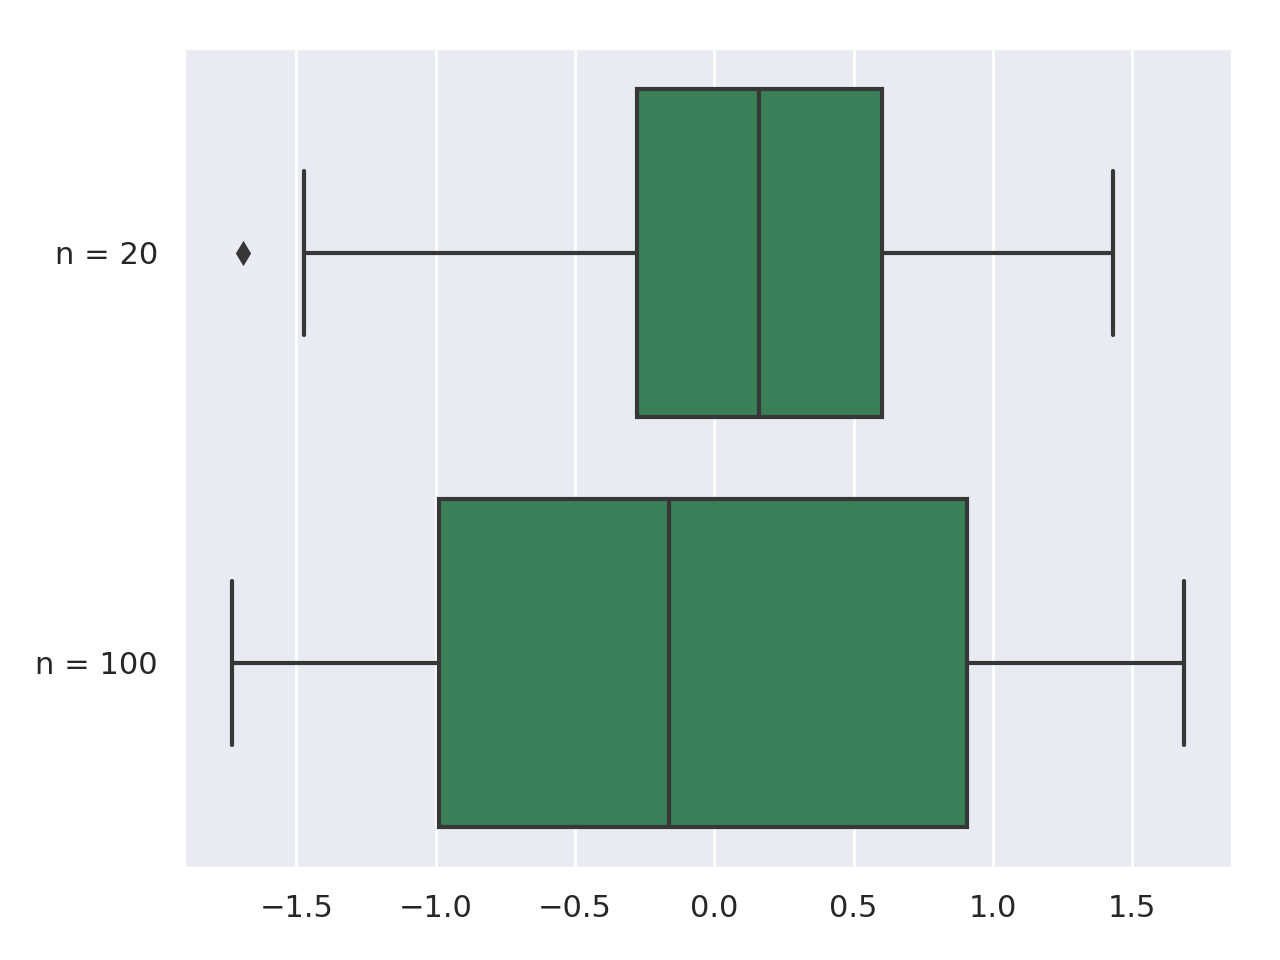
\includegraphics[width=12.cm, height=9.cm]{unif}}
\label{2_pic:2}
\caption{Боксплот Тьюки для выборок из равномерного распределения}
\end{figure}

\threeimage{em_uni_20}{em_uni_60}{em_uni_100}{равномерного распределения}
\triplethreeimage{ker_uni_20}{ker_uni_60}{ker_uni_100}{равномерного распределения}

\newpage
\textbf{Распределение Коши} с параметрами 0, 1

\begin{figure}[h!]
	\centering
	\center{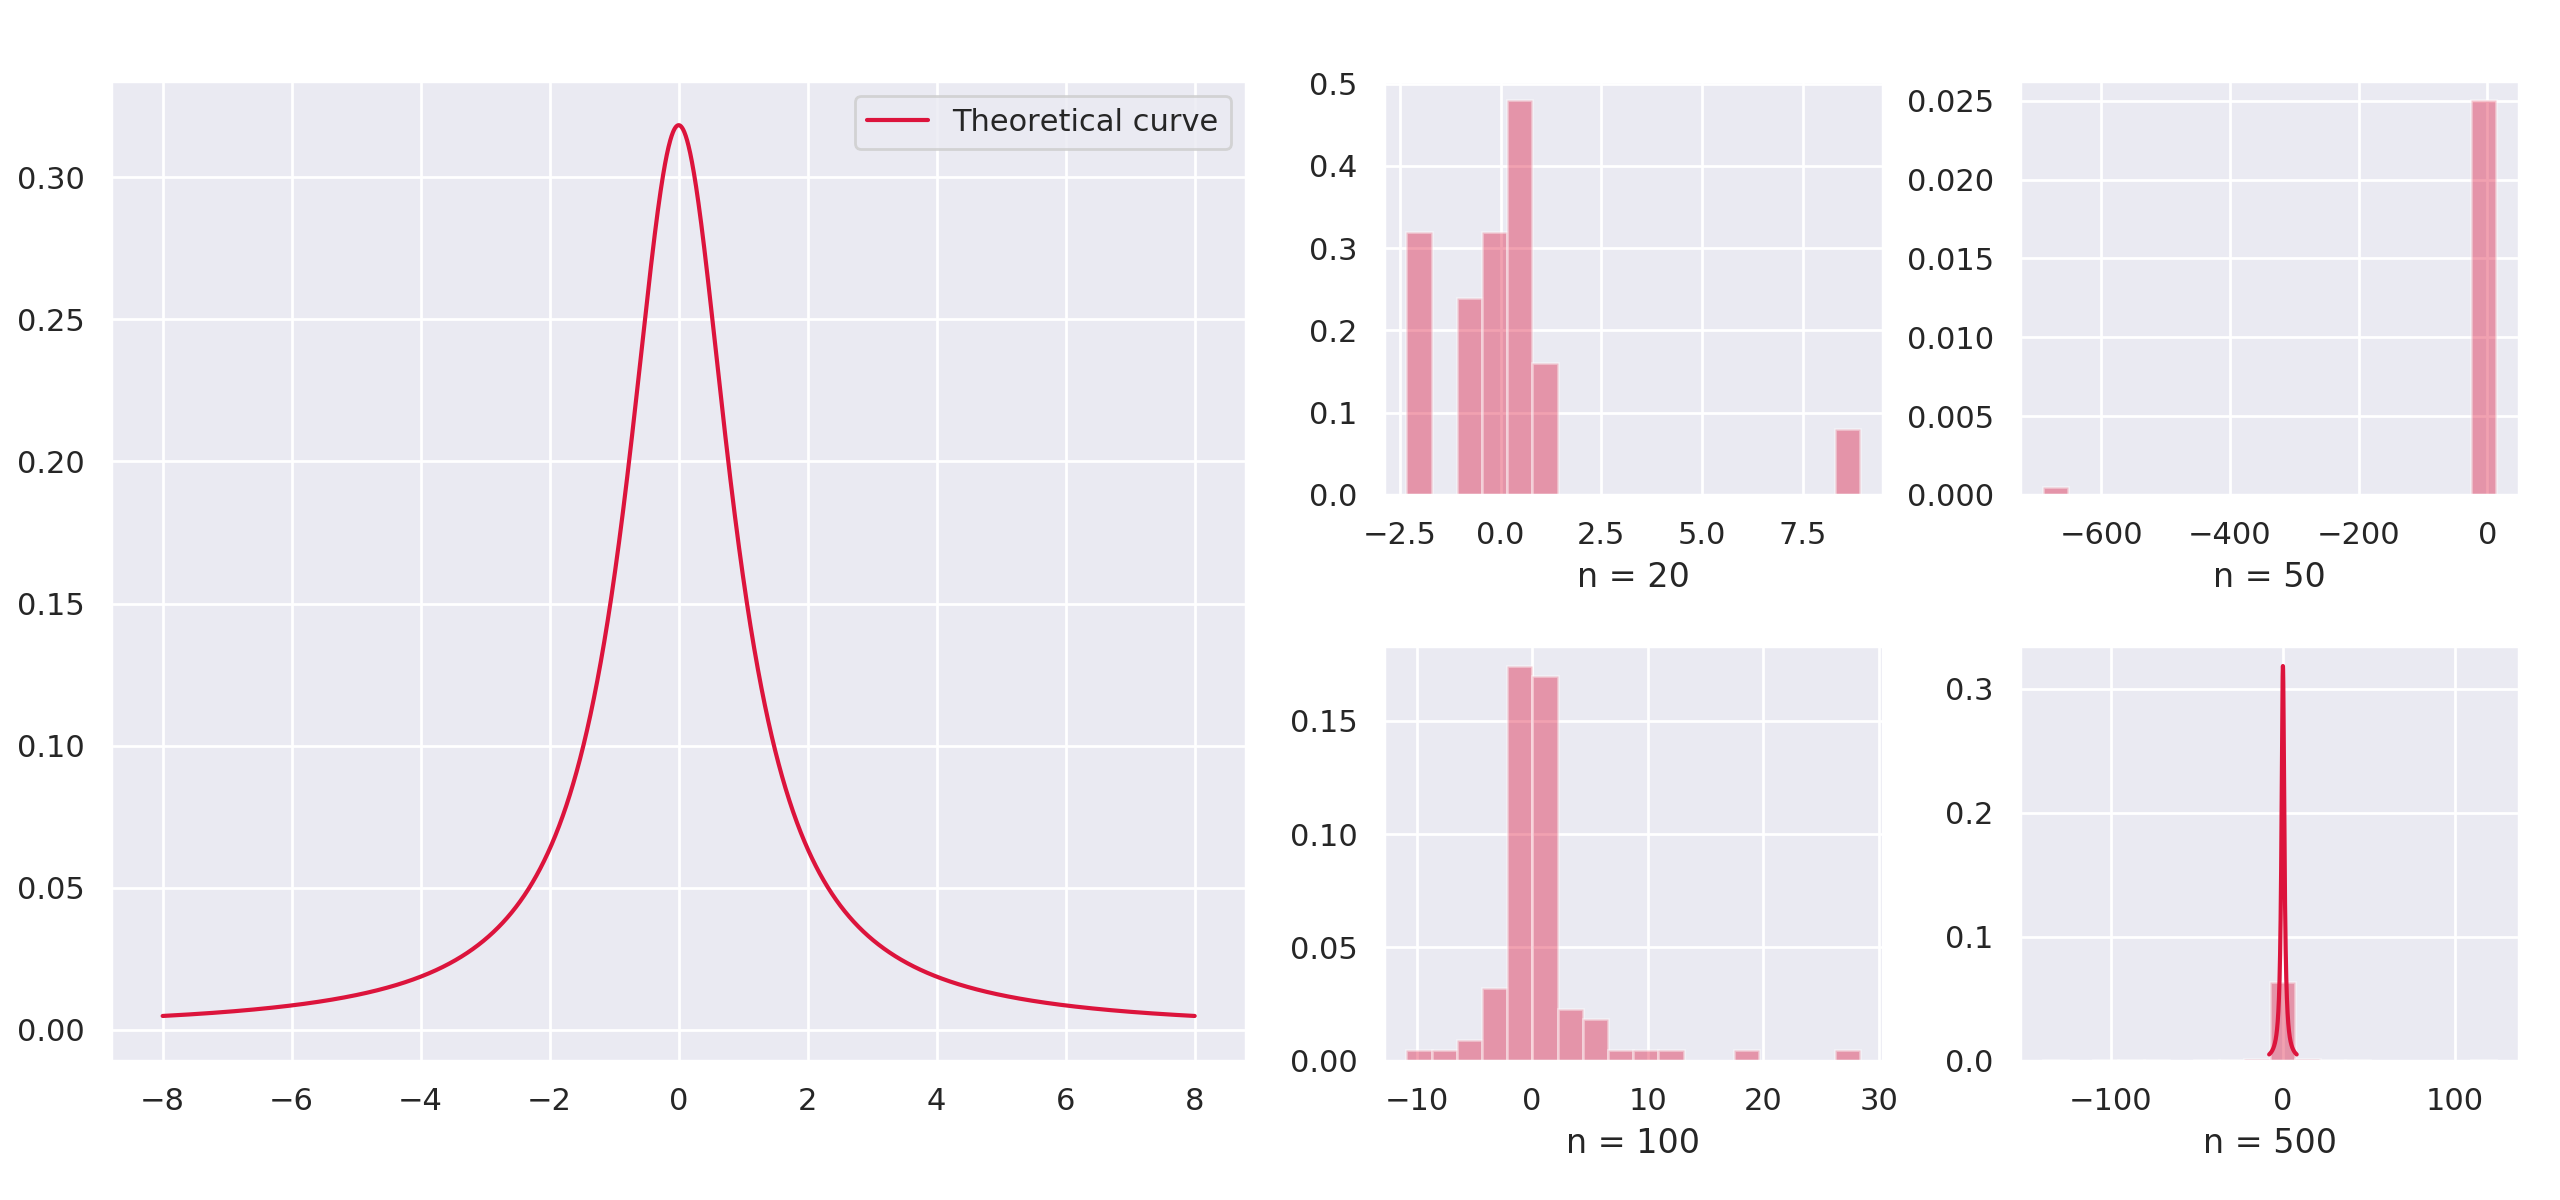
\includegraphics[width=16.8cm, height=8.5cm]{cauchy_th}}
	\caption{Гистограмма распределения Коши}
	\label{3_pic:1}
\end{figure}

\begin{table}[h!]
	\begin{tabular}{ | c | c | c | c | c | c |}
	\hline
	$n = 20$ & $\overline{x}$ & $med\;x$ & $z_R$ & $z_Q$ & $z_{tr}$ \\ \hline
	$E(z)$ & -4.1847 & -0.0185 & -41.9652 & -0.0013 & 0.0043 \\ \hline
	$D(z)$ & $10^4$ & 0.1450 & $10^6$ & 0.3753 & 0.4334 \\ \hline
	\end{tabular}
	\\
	\\ \\ 
	\begin{tabular}{ | c | c | c | c | c | c |}
	\hline
	$n = 50$ & $\overline{x}$ & $med\;x$ & $z_R$ & $z_Q$ & $z_{tr}$ \\ \hline
	$E(z)$ & 3.7413 & 0.0051 & 95.1768 & -0.0011 & -0.0022 \\ \hline
	$D(z)$ & $10^4$ & 0.0483 & $10^7$ & 0.1102 & 0.1094 \\ \hline
	\end{tabular}
	\\
	\\ \\ 
	\begin{tabular}{ | c | c | c | c | c | c |}
	\hline
	$n = 100$ & $\overline{x}$ & $med\;x$ & $z_R$ & $z_Q$ & $z_{tr}$ \\ \hline
	$E(z)$ & 2.6928 & -0.0082 & 133.6930 & -0.0080 & -0.0116 \\ \hline
	$D(z)$ & $10^3$ & 0.0247 & $10^8$ & 0.0522 & 0.0513 \\ \hline
	\end{tabular}
	\caption*{Таблицы моментов 1-го и 2-го порядков}
	\indent{}\\
	\indent{Соотношение дисперсий при $n = 100$: $\;med\;x < z_{tr} < z_Q < \overline{x} < z_R$}
\end{table}
\begin{center}
    \begin{tabular}{ c | c | c }
        $$ & Практическая доля выбросов & Теоретическая доля выбросов  \\ \hline
        $n = 20$ & 0.15 & 0.15 \\ \hline
        $n = 100$ & 0.15 & 0.15 \\ 
    \end{tabular}
\end{center}

\begin{figure}[h!]
\centering
\center{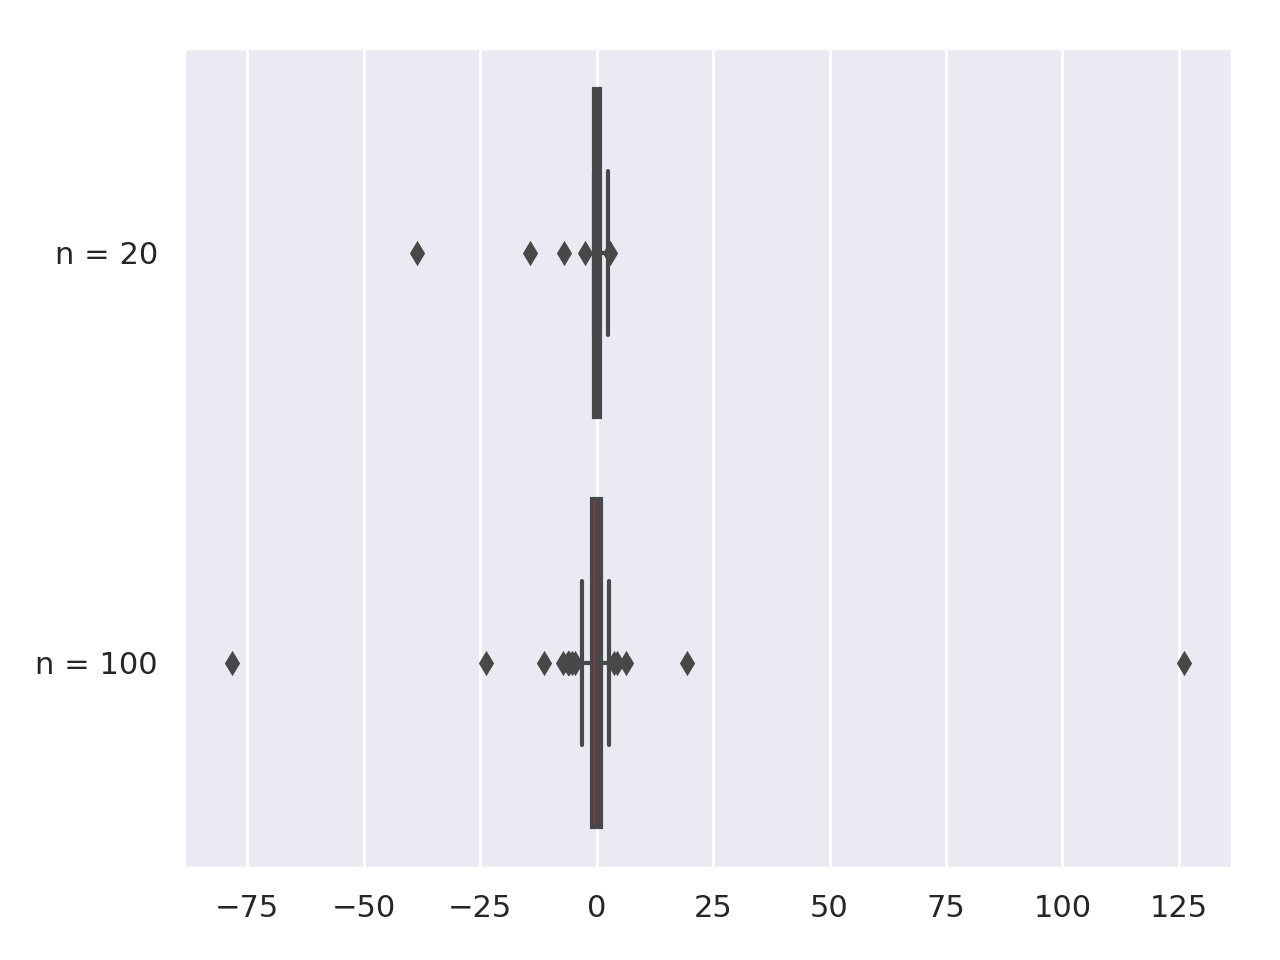
\includegraphics[width=12.cm, height=9.cm]{cauch}}
\label{3_pic:2}
\caption{Боксплот Тьюки для выборок из распределения Коши}
\end{figure}
\threeimage{em_cauch_20}{em_cauch_60}{em_cauch_100}{распределения Коши}
\triplethreeimage{ker_cauch_20}{ker_cauch_60}{ker_cauch_100}{распределения Коши}

\newpage
\textbf{Распределение Лапласа} с параметрами 0, $\frac{1}{\sqrt{2}}$

\begin{figure}[h!]
	\centering
	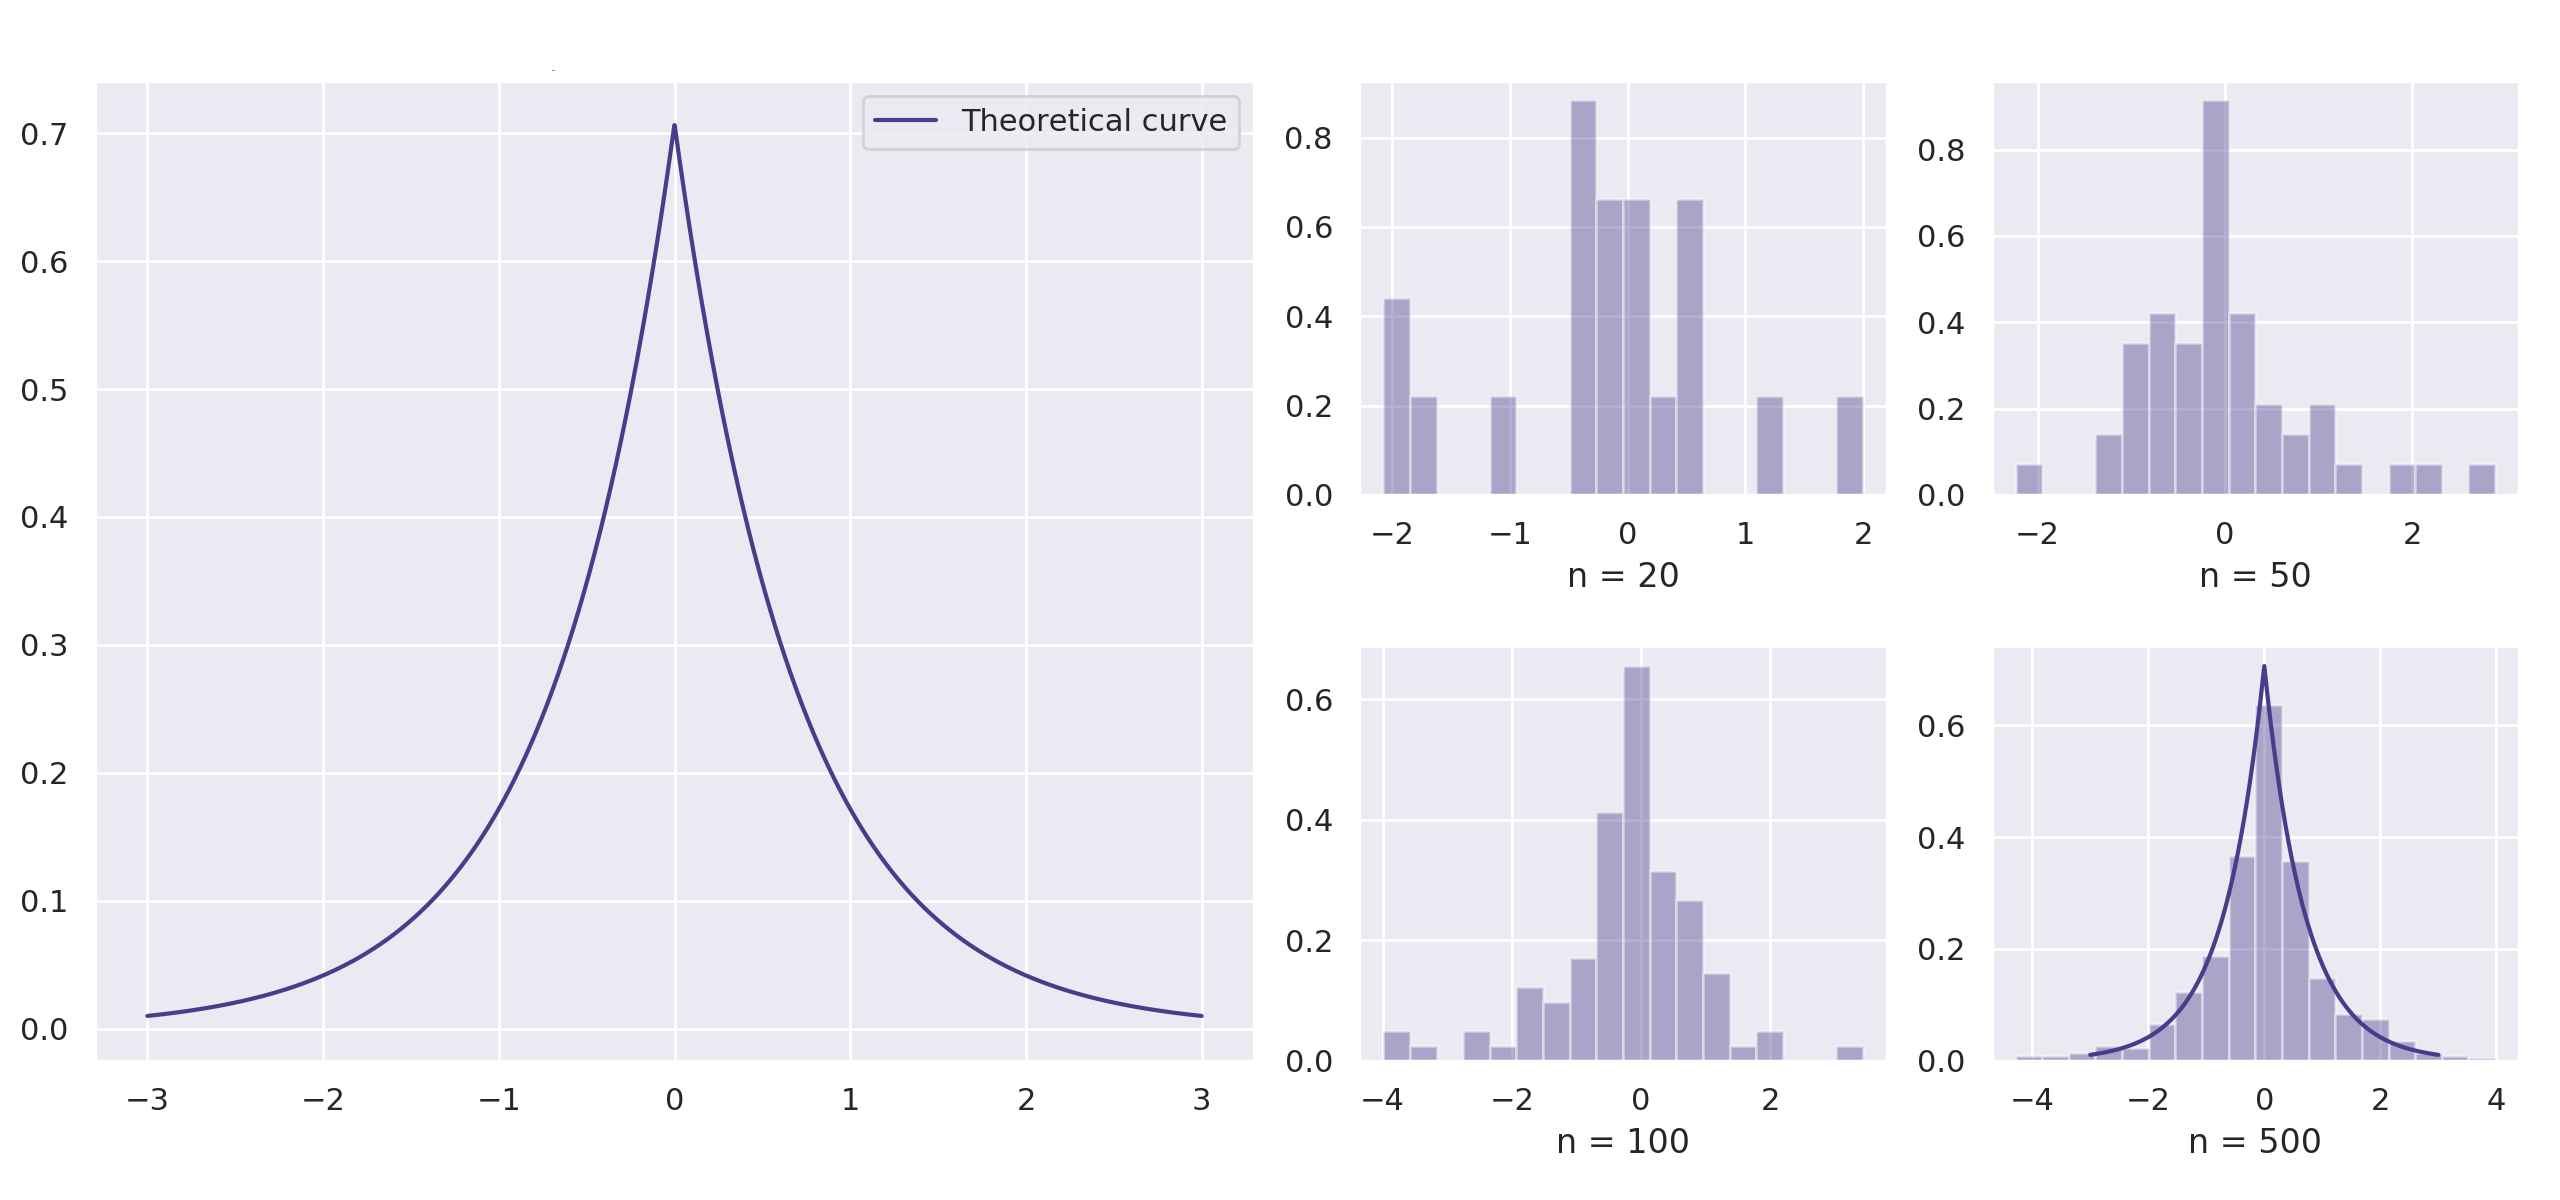
\includegraphics[width=16.8cm, height=8.5cm]{laplace_th}
	\caption{Гистограмма рампределения Лапласа}
	\label{4_pic:1}
\end{figure}

\begin{table}[h!]
	\begin{tabular}{ | c | c | c | c | c | c |}
	\hline
	$n = 20$ & $\overline{x}$ & $med\;x$ & $z_R$ & $z_Q$ & $z_{tr}$ \\ \hline
	$E(z)$ & -0.0113 & -0.0035 & -0.0344 & -0.0087 & -0.0070 \\ \hline
	$D(z)$ & 0.0550 & 0.0348 & 0.4406 & 0.0519 & 0.0427 \\ \hline
	\end{tabular}
	\\
	\\ \\ 
	\begin{tabular}{ | c | c | c | c | c | c |}
	\hline
	$n = 50$ & $\overline{x}$ & $med\;x$ & $z_R$ & $z_Q$ & $z_{tr}$ \\ \hline
	$E(z)$ & 0.0028 & -0.0010 & 0.0085 & 0.0035 & 0.0019 \\ \hline
	$D(z)$ & 0.0193 & 0.0130 & 0.3839 & 0.0206 & 0.0156 \\ \hline
	\end{tabular}
	\\
	\\ \\ 
	\begin{tabular}{ | c | c | c | c | c | c |}
	\hline
	$n = 100$ & $\overline{x}$ & $med\;x$ & $z_R$ & $z_Q$ & $z_{tr}$ \\ \hline
	$E(z)$ & -0.0059 & -0.0029 & -0.0104 & -0.0047 & -0.0051 \\ \hline
	$D(z)$ & 0.0097 & 0.0056 & 0.3931 & 0.0093 & 0.0071 \\ \hline
	\end{tabular}
	\caption*{Таблицы моментов 1-го и 2-го порядков}
	\indent{}\\
	\indent{Соотношение дисперсий при $n = 100$: $\;med\;x < z_{tr} < z_Q < \overline{x} < z_R$}
\end{table}

\begin{center}
    \begin{tabular}{ c | c | c }
        $$ & Практическая доля выбросов & Теоретическая доля выбросов  \\ \hline
        $n = 20$ & 0.07 & 0.06 \\ \hline
        $n = 100$ & 0.06 & 0.06 \\ 
    \end{tabular}
\end{center}

\begin{figure}[h!]
\centering
\center{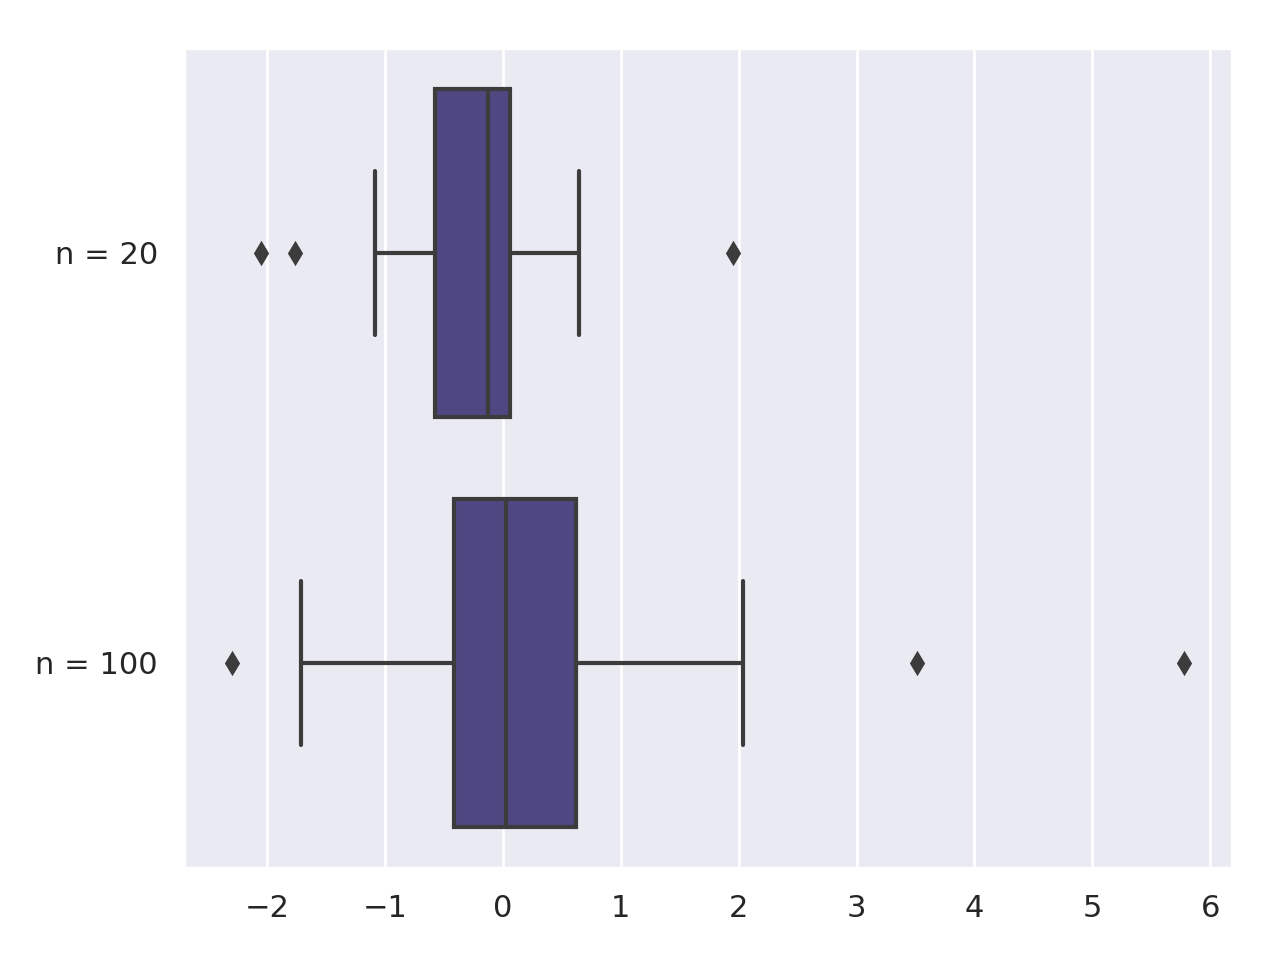
\includegraphics[width=12.cm, height=9.cm]{laplace}}
\label{4_pic:2}
\caption{Боксплот Тьюки для выборок из распределения Лапласа}
\end{figure}
\threeimage{em_lap_20}{em_lap_60}{em_lap_100}{распределения Лапласа}
\triplethreeimage{ker_lap_20}{ker_lap_60}{ker_lap_100}{распределения Лапласа}

\newpage
\textbf{Распределение Пуассона} с параметром $\lambda = 7$  

\begin{figure}[h!]
	\centering
	\center{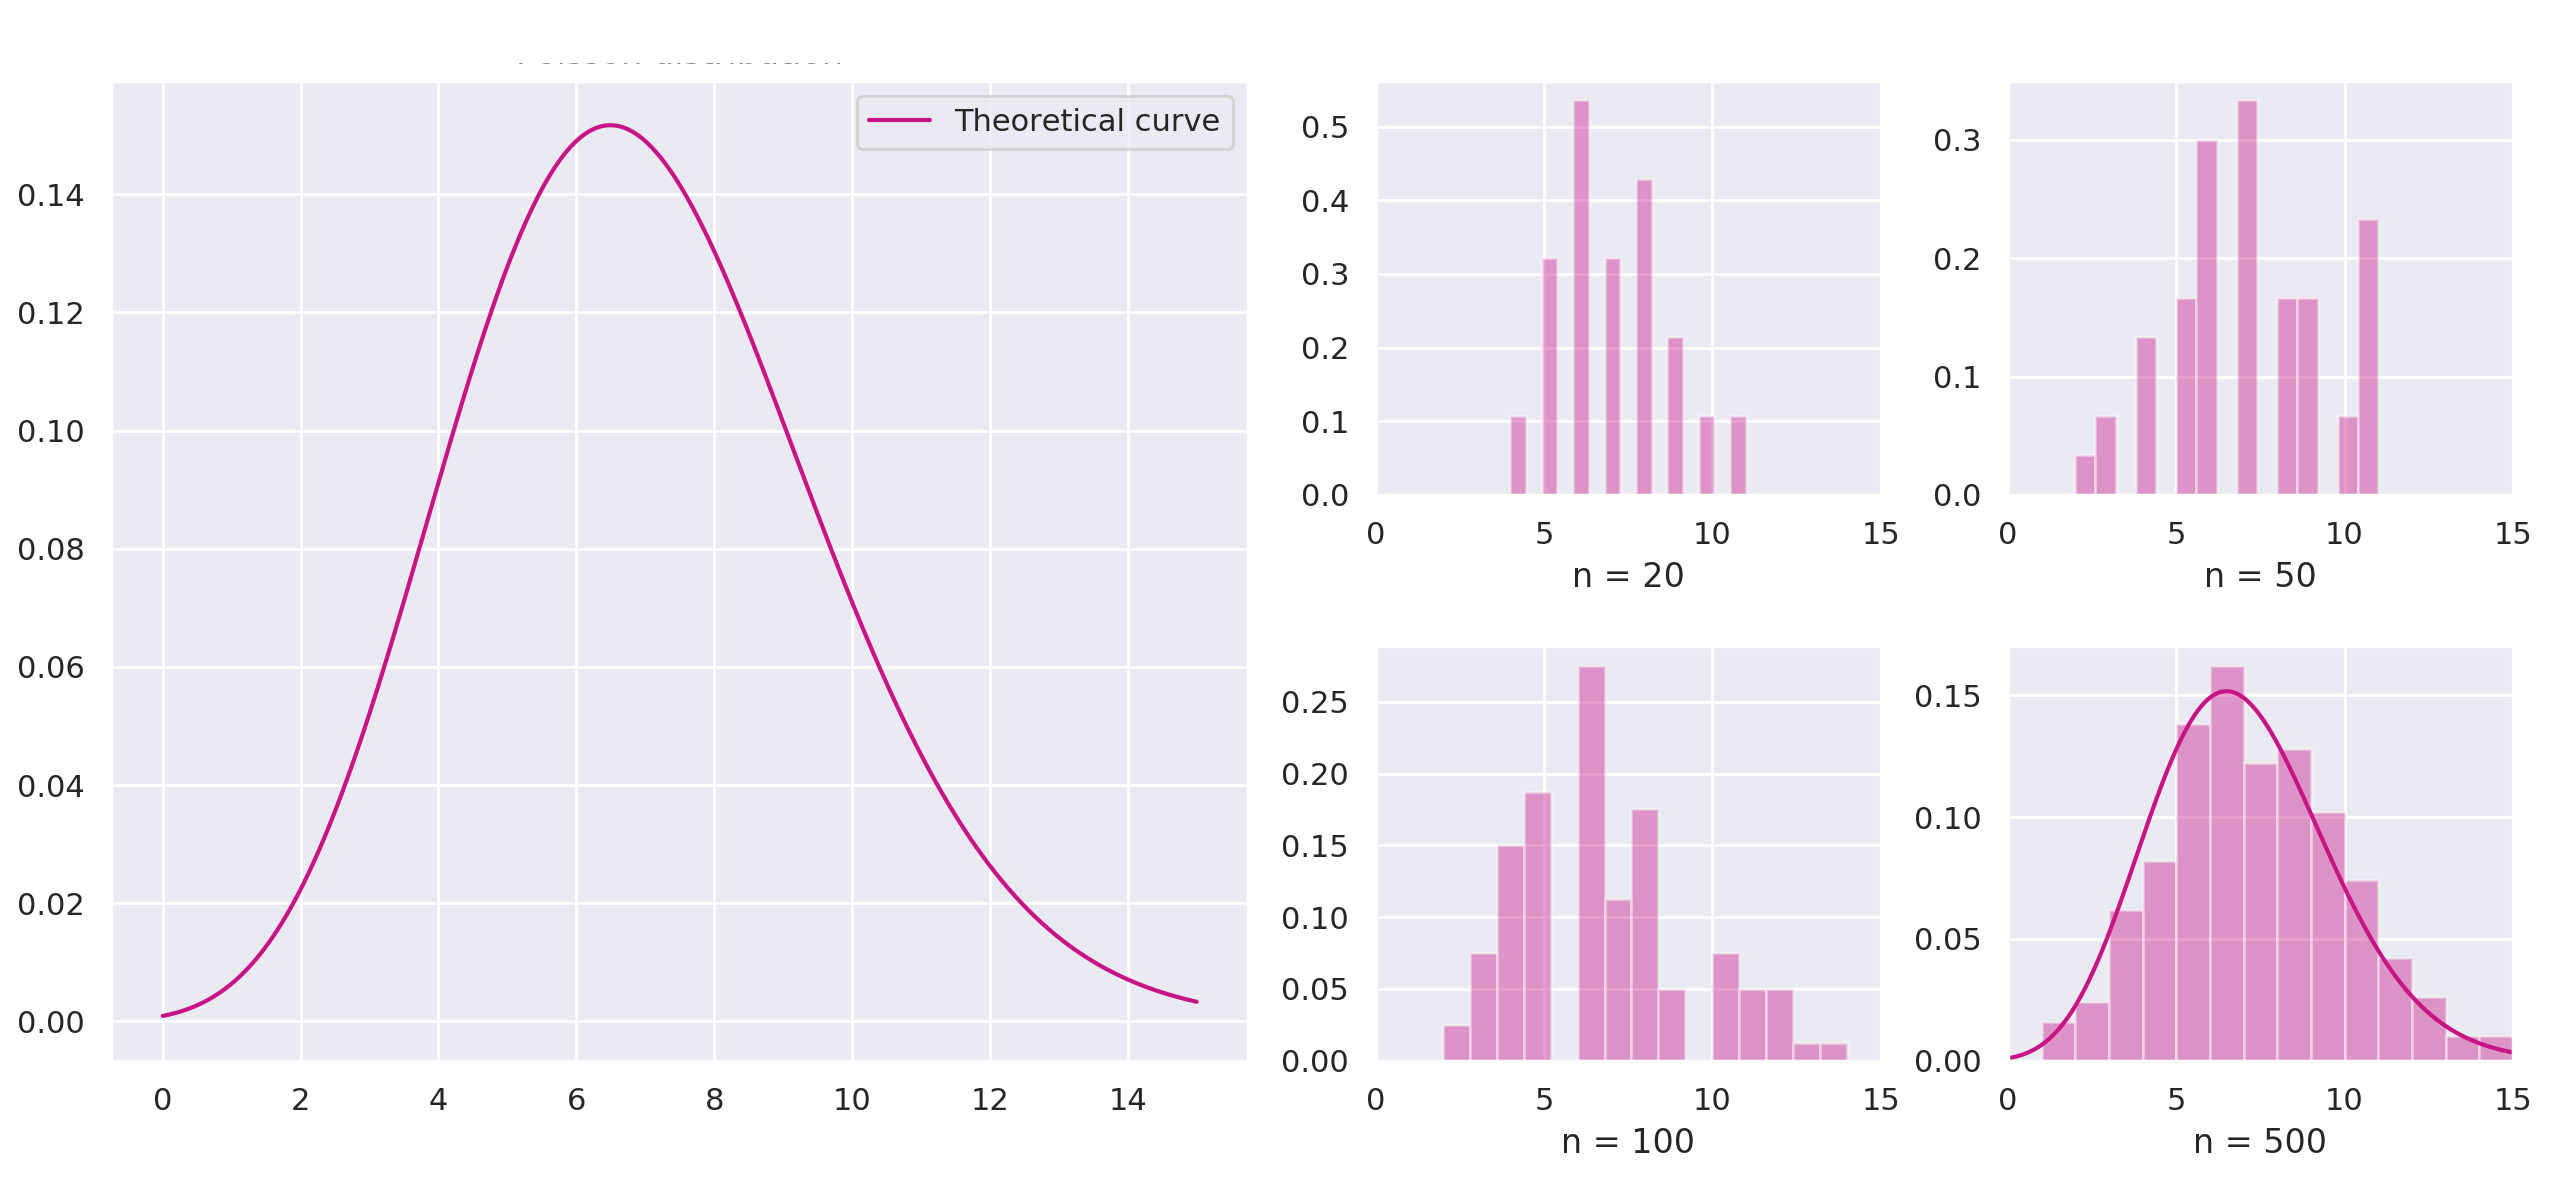
\includegraphics[width=16.cm, height=7.6cm]{poisson_th}}
	\caption{Гистограмма рампределения Пуассона}
	\label{5_pic:1}
\end{figure}

\begin{table}[h!]
	\begin{tabular}{ | c | c | c | c | c | c |}
	\hline
	$n = 20$ & $\overline{x}$ & $med\;x$ & $z_R$ & $z_Q$ & $z_{tr}$ \\ \hline
	$E(z)$ & 6.9844 & 6.8310 & 7.4820 & 6.9067 & 6.8978 \\ \hline
	$D(z)$ & 0.3285 & 0.5259 & 1.0587 & 0.4049 & 0.3441 \\ \hline
	\end{tabular}
	\\
	\\ \\ 
	\begin{tabular}{ | c | c | c | c | c | c |}
	\hline
	$n = 50$ & $\overline{x}$ & $med\;x$ & $z_R$ & $z_Q$ & $z_{tr}$ \\ \hline
	$E(z)$ & 7.0165 & 6.8640 & 7.7515 & 6.9400 & 6.9287 \\ \hline
	$D(z)$ & 0.1561 & 0.2665 & 0.8315 & 0.2299 & 0.1639 \\ \hline
	\end{tabular}
	\\
	\\ \\ 
	\begin{tabular}{ | c | c | c | c | c | c |}
	\hline
	$n = 100$ & $\overline{x}$ & $med\;x$ & $z_R$ & $z_Q$ & $z_{tr}$ \\ \hline
	$E(z)$ & 7.0063 & 6.8755 & 7.9230 & 6.9088 & 6.9181 \\ \hline
	$D(z)$ & 0.0714 & 0.1482 & 0.7266 & 0.1074 & 0.0746 \\ \hline
	\end{tabular}
	\caption*{Таблицы моментов 1-го и 2-го порядков}
	\indent{}\\
	\indent{Соотношение дисперсий при $n = 100$: $ \overline{x} < z_{tr} < z_Q < med\;x < z_R$}\\
\end{table}

\begin{center}
    \begin{tabular}{ c | c | c }
        $$ & Практическая доля выбросов & Теоретическая доля выбросов  \\ \hline
        $n = 20$ & 0.027 & 0.003 \\ \hline
        $n = 100$ & 0.012 & 0.002 \\ 
    \end{tabular}
\end{center}
\begin{figure}[h!]
\centering
\center{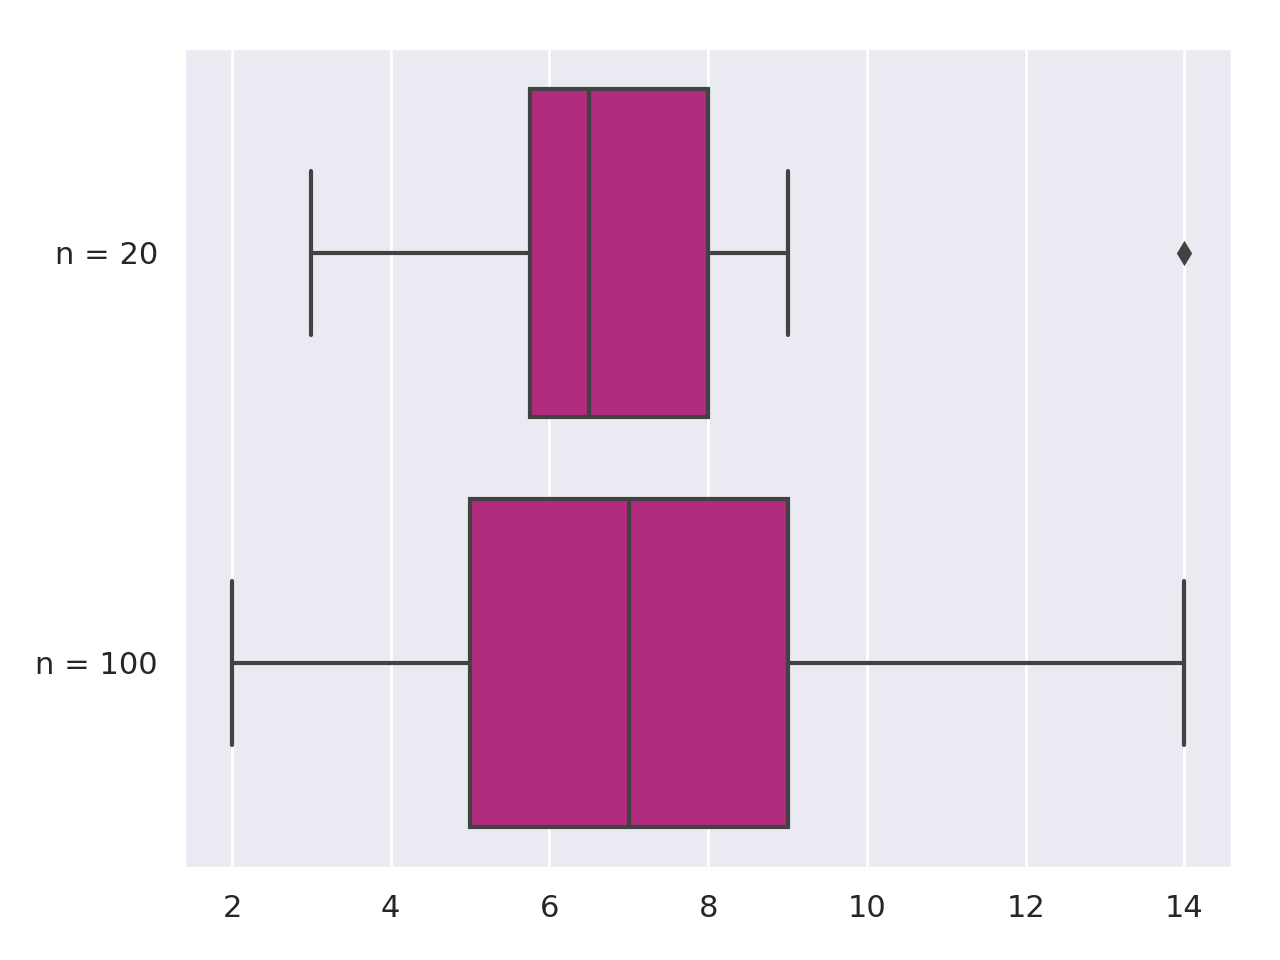
\includegraphics[width=12.cm, height=8.5cm]{poiss}}
\label{5_pic:2}
\caption{Боксплот Тьюки для выборок из распределения Пуассона}
\end{figure}

\threeimage{em_pois_20}{em_pois_60}{em_pois_100}{распределения Пуассона с параметром $\lambda = 2$}
\triplethreeimage{ker_pois_20}{ker_pois_60}{ker_pois_100}{распределения Пуассона $\lambda = 2$}

\newpage
\indent{ Выбор параметра обоснован стремлением распределения к нормальному при увеличении $\lambda$. Для наглядной визуализации  подходит число 7, к тому же являющееся числом Миллера, или предельной порцией информации, обрабатываемой человеком за раз (оригинальная статья - \cite{ms_2}). Этот факт является довольно символичным, учитывая область применения распределения Пуассона. Чтобы построить эмпирическую функцию распределения и ядерную оценку плотности на указанном отрезке, будем использовать $\lambda = 2$.}

\section*{Выводы}
\addcontentsline{toc}{section}{Выводы}
\indent{ \indentПри достаточной мощности выборки из распределений (n = 100) гистограмму можно рассматривать как аналог плотности распределения непрерывной случайной величины.}

\indent{По полученным соотношениям дисперсий выборок из распределений можно сделать вывод о том, что полусумма экстремальных значений $z_R$ имеет наибольший разброс относительно математического ожидания. Данное суждение не сходится с результатами для случая равномерного распределения на отрезке. Медиана равномерного распределения на $[a, b]$ есть $med = \frac{a+b}{2}$, что и является полусуммой значений в крайних точках отрезка.}\\
\indent{Также в случае симметричного распределения, исходя из дисперсий, наиболее выгодно использовать выборочное среднее, чем медиану, хотя они и оценивают одну и ту же величину в данном случае. Но для распределения Лапласа медиана становится более эффективной.}\\
\indent{Дисперсии таких характеристик, как усеченное среднее или полусумма квартилей, показывают среднее отклонение относительно остальных. Усеченное среднее представляет собой некий баланс между медианой и выборочным средним (является ими в частных случаях параметра $\alpha$)}

\indent{Взглянув на полученные боксплоты Тьюки, можно сделать вывод о том, что равномерное распределение не имеет выбросов. Ненулевое значение в малой выборке при расчете квантилей с использованием значений выборки есть показатель того, что нельзя судить о характере распределения по выборке размером $n = 20$ окончательно. Отсутствие выбросов объясняется тем, что функция плотности такого респределения постоянна, и элемент выборки никогда будет вне отрезка, ограниченного \eqref{3_eq:1}, \eqref{3_eq:2}}

\indent{Наибольший процент выбросов установлен для выборов из распределения Коши. Также увеличение выборки не влияет на изменение результата, математического ожидания нет. Обратимся к результатам предыдущей лабораторной работы. Дисперсия размаха распределения принимает значения порядка $10^8$. Это объясняет тот факт, что доля выбросов достаточно высока. Распределение Коши имеет тяжелые хвосты, и доля элементов, принимающих далекие от центра распределения значения, на порядок выше по сравнению с остальными распределениями, такими как нормальное, Лапласа, Пуассона.}

\indent{ Описывая полученные статистические функции, можно заключить, что чем больше выборка, тем точнее эмпирическая функция распределения оценивает теоретическую.}

\indent{ Точность ядерной оценки плотности сильно варьируется в зависимости от значения сглаживающего параметра $h$. Так, при $h \to 0$ оценка плотности точна на выборочных данных, но только на них, и такая функция не способна описать характер распределения. Выбрав $(n + 1)$-ое значение из распределения, мы можем столкнуться с тем, что статистическая функция плохо оценит значение теоретической функции плотности вероятности для данного выборочного элемента. В таком случае можно говорить о плохой способности функции к обобщению.}

\indent{ Напротив, при увеличении параметра $h$ ядерная оценка плотности может показывать себя плохо даже на выборочных данных и вообще не позволяет понять характера распределения.}

\indent{ Выбор параметра сглаживания следует производить исходя из того, насколько плотно распределение объектов выборки; большей плотности соответствует выбор меньшего параметра и наоборот.}

%%%%%%%%%%%%%%%%%%%%%%%%%%%%%%%%%%%%%%%%%%

\newpage
\begin{thebibliography}{}
	\bibitem{ms_1} \textit{Кадырова Н. О.} Теория вероятностей и математическая статистика. Статистический анализ данных: учеб. пособие / \textit{Н. О. Кадырова, Л. В. Павлова, И. Е. Ануфриев.} - СПб.: Изд-во Политехн. ун-та, 2010. -54с.
	\bibitem{ms_2} \textit{Miller, G. A.} The magical number seven, plus or minus two: Some limits on our capacity for processing information. Psychological Review. 1956; 63:81–97.
    \bibitem{ms_3}\textit{Chrisman, L.} How the strange Cauchy distribution proved useful. \textit{Lumina Decision Systems} (2018). URL: http://www.lumina.com/blog/how-the-strange-cauchy-distribution-proved-useful
    \bibitem{ms_4}\textit{Conlen, M.} Kernel Density Estimation (2019). URL: https://mathisonian.github.io/kde/
\end{thebibliography}


\end{document}{}